\documentclass[a4paper,12pt]{article}

\usepackage[pdftex]{graphicx}

\newcommand{\menu}[2]{{\it \vskip2mm #1 $\rightarrow$ #2 \vskip2mm}}
\newcommand{\dynmenu}[3]{{\it \vskip2mm #1 $\rightarrow$ #2 $\rightarrow$ #3 \vskip2mm}}

\title{ElmerGUI manual v. 0.2}
\author{Mikko Lyly}

\begin{document}
\maketitle

\newpage

\tableofcontents

\newpage

\section{Introduction}

ElmerGUI is a graphical user interface for the Elmer software suite
\cite{ElmerHome}. The program is capable of importing finite element mesh files in
various formats, generating finite element partitionings for models with piecewise
linear boundaries, setting up PDE-systems to solve, and exporting model data and results
for ElmerSolver and ElmerPost to visualize. There is also an internal postprocessor,
which can be used as an alternative to ElmerPost, to draw color surfaces, contours, 
vector fields, and visualize time dependent data.

\begin{figure}[ht]
\begin{center}
 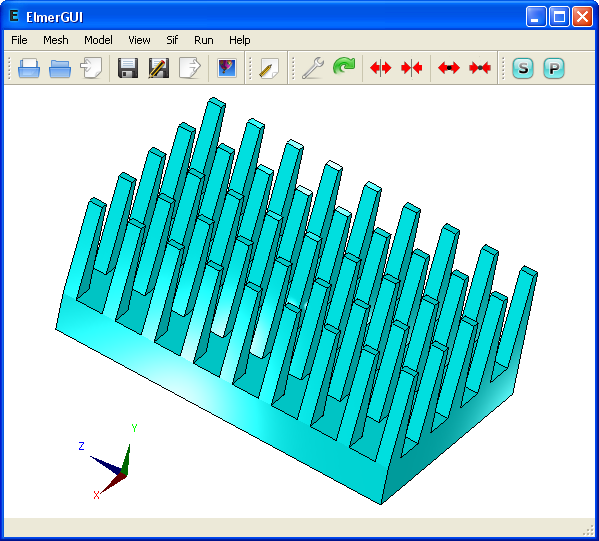
\includegraphics[scale=0.5]{images/elmergui.png}
\caption{Main window of ElmerGUI.}
\end{center}
\end{figure}

One of the main features of ElmerGUI is the interface to the parallel solver,  {\tt ElmerSolver\_mpi}.
The GUI hides from the user a number of operations that are normally performed from command line with various external tools related to domain decomposition, launching the paralle processes, and merging the results. This makes it possible to use ElmerSolver with multi-core processors even on interactive desktop
environments.

The menus of ElmerGUI are programmable and it is relatively easy to strip and customize the interface
for an proprietary application. An example of customizing the menus is provided in appendix A.

ElmerGUI relies on the Qt4 cross platform framework from Trolltech \cite{QtHome}, and it uses the Qwt5
libray by Josef Wilgen and Uwe Rathman\cite{QwtHome}. The internal postprocessor is based on the VTK  library of Ken Martin, Will Schroeder, and Bill Lorensen \cite{VTKHome}. The CAD import features are
implemented by linking against the OCC library from OpenCASCADE S.A.S. \cite{OCCHome}. The program is
also capable of using Tetgen \cite{TetgenHome} and Netgen \cite{NetgenHome} as external finite element
mesh generators.

\section{Installation from source}

The source code of ElmerGUI is available from the subversion repository of SourceForge.Net. The GPL
licenced source may be downloaded by executing the following command with a SVN client program(on
Windows the Tortoise SVN client is recommended):

\begin{footnotesize}
\begin{verbatim}
svn co https://elmerfem.svn.sourceforge.net/svnroot/elmerfem/trunk trunk
\end{verbatim}
\end{footnotesize}
\noindent This will retrieve the current development version of the whole Elmer-suite.

\subsection{Linux}

Bofore staring to compile, please make sure that you have the development package of Qt 4
installed on your system (i.e., libraries, headers, and program development tools). Qt version 4.2
or newer is recommended. You may also wish to install Qwt 5, VTK version 5, and OpenCASCADE 6.3, 
for additional functionality.

The program is compiled and installed by executing the following sequence of commands in a terminal window:
\begin{verbatim}
$ cd elmerfem/trunk/ElmerGUI
$ qmake
$ make
$ make install
\end{verbatim}
The default installation directory defined in the project file {\tt ElmerGUI.pro} is
{\tt /usr/local/bin}.

It is possible that the project file ``ElmerGUI.pro'' needs to be edited depending on how and
where the external libraries have been installed. The lines that need attention can be found from
the beginning of the file.

Once the build process has finished, it suffices to set up the environment variable {\tt ELMERGUI\_HOME}
and add it to {\tt PATH}:
\begin{verbatim}
$ export ELMERGUI_HOME=/usr/local/bin
$ export PATH=$PATH:$ELMERGUI_HOME
\end{verbatim}
The program is started by entering the command
\begin{verbatim}
$ ElmerGUI
\end{verbatim}

Later, it is possible to upgrade ElmerGUI by typing the following commands within the build directory:
\begin{verbatim}
$ svn update
$ make install
\end{verbatim}

\subsection{Windows}

On 32-bit Windows systems, it is possible to use precompiled binary packages, which are distributed
through the file release system of SourceForge.NET \cite{ElmerfemHome}. The binary packages may depend
on external components, which must be installed prior to downloading Elmer. The list of possible
dependencies can be found from the ``Release notes'' of the file release.

It is also possible to compile ElmerGUI from source. This can be done either with Visual Studio
2008 C++ Express Edition \cite{VCEE2008Home}, or by using the MinGW compiler suite \cite{MinGWHome}.

The compilation instructions for MinGW are more or less the same as for Linux. The only exception
is that then OCC should probably be excluded from compilation, and the cad import functionality will
be unavailable. The advantage of using MinGW, on the other hand, is that it is then possible to use
Qt's precompiled binary packages \cite{QtHome}, which otherwise have to be built from source. MinGW
might also be the natural choice for users that prefer Unix-like operating environments.

The easiest way to compile ElmerGUI with VC++ is to invoke ``Visual Studio 2008 Command Prompt''
and execute the following sequence commands within ElmerGUI's source directory:
\begin{verbatim}
> qmake
> nmake
> nmake install
\end{verbatim}

Again, it is necessary to verify that the paths to all external components have been correctly
defined in ``ElmerGUI.pro''. The build process is performed in release mode, producing the
executable ``ElmerGUI.exe''.

The final task is to introduce the environment variable {\tt ELMERGUI\_HOME} and add it to the
binary search path.

\section{Input files}

\subsection{Geometry input files and mesh generation}

ElmerGUI is capable of importing finite element mesh files and generating two or three
dimensional finite element partitionings for bounded domains with piecewise linear
boundaries. It is possible to use one of the following mesh generators:
\begin{itemize}
 \item ElmerGrid (built-in)
 \item Tetgen (optional)
 \item Netgen (optional)
\end{itemize}
The default import filter and mesh generator is ElmerGrid. Tetgen and Netgen are optional
modules, which may or may not be available depending on the installation (installation and
compilation instructions can be found from Elmer's source tree in {\tt trunk/misc})

An import filter or a mesh generator is selected automatically by ElmerGUI when a geometry
input file is opened from the File menu:

\menu{File}{Open...}

The selection is based on the input file suffix according to Table 1. If two or more
generators are capable of handing the same format, then the user defined ``preferred
generator'' will be used. The preferred generator is defined in

\menu{Mesh}{Configure...}

Once the input file has been opened, it is possible to modify the mesh parameters
and remesh the geometry for better accuracy or computational efficiency. The mesh parameters
can be found from the same place as the preferred generator. The control string for Tetgen
has been discussed and explained in detail in \cite{TetgenHome}.

\begin{center}
\begin{tabular}{|c|c|c|c|}
\hline
 Suffix & ElmerGrid & Tetgen & Netgen \\
\hline 
.FDNEUT & yes & no & no \\
.grd  & yes & no & no \\
.msh & yes & no & no \\
.mphtxt & yes & no & no \\
.off & no & yes & no \\
.ply & no & yes & no \\
.poly & no & yes & no \\
.smesh & no & yes & no \\
.stl  & no & yes & yes \\
.unv & no & yes & no \\
\hline
\end{tabular}
\vskip5mm
Table 1. Input files and capabilities of the mesh generators.
\end{center}

The mesh generator is reactivated from the Mesh menu by choosing

\menu{Mesh}{Remesh}
\noindent In case of problems, the meshing thread may be terminated by executing 
\menu{Mesh}{Terminate meshing}

\subsection{Elmer mesh files}

An Elmer mesh consists of the following four text files (detailed description of the file format can be found from Appendix B):

\begin{footnotesize}
\begin{verbatim}
mesh.header 
mesh.nodes 
mesh.elements 
mesh.boundary 
\end{verbatim}
\end{footnotesize}

\noindent These files have to reside in the same mesh directory.

Elmer mesh files may be loaded and/or saved by opening the mesh directory from the File menu:
\menu{File}{Load mesh...}
\noindent and/or
\menu{File}{Save as...}

\subsection{Project files}

An ElmerGUI project consists of a project directory containing Elmer mesh files and an xml-formatted 
document {\tt egproject.xml} describing the current state and settings. Projects may be loaded and/or saved from the File menu as
\menu{File}{Load project...}
\noindent and/or
\menu{File}{Save project...}

When an ElmerGUI project is loaded, a new solver input file will be generated and saved
in the project directory using the sif-name defined in
\menu{Model}{Setup...}
\noindent If there is an old solver input file with the same name, it will be overwritten.

The contents of a typical project directory is the following:

\begin{footnotesize}
\begin{verbatim}
case.sif 
egproject.xml
ELMERSOLVER_STARTINFO 
mesh.boundary 
mesh.elements 
mesh.header 
mesh.nodes
\end{verbatim}
\end{footnotesize}

\section{Model definitions}

\subsection{Setup menu}

The general setup menu can be found from
\menu{Model}{Setup...}
\noindent This menu defines the basic variables for the ``Header'', ``Simulation'',
and ``Constants'' blocks for a solver input file. The contents of these blocks have
been discussed in detail in the SolverManual of Elmer \cite{ElmerHome}.

\begin{figure}[ht]
\begin{center}
 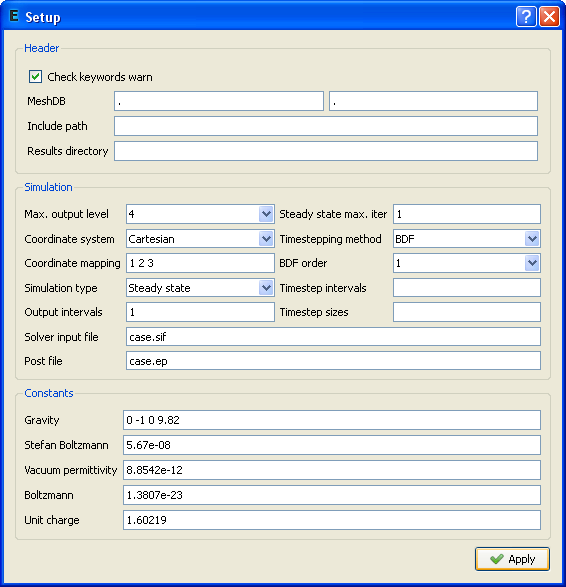
\includegraphics[scale=0.5]{images/setupmenu.png}
\caption{Setup menu.}
\end{center}
\end{figure}

\subsection{Equation menu}

The first ``dynamical menu'' constructed from the ElmerGUI definition files (see Appendix A) is
\menu{Model}{Equation}
\noindent This menu defines the PDE-system to be solved as well as the numerical
methods and parameters used in the solution. It will be used to generate the ``Solver''
blocks in a solver input file.

A PDE-system (a.k.a ``Equation'') is defined by choosing
\dynmenu{Model}{Equation}{Add...}

\begin{figure}[ht]
\begin{center}
 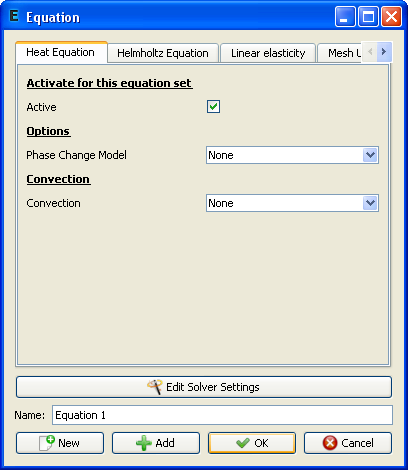
\includegraphics[scale=0.5]{images/equation.png}
\caption{Equation menu.}
\end{center}
\end{figure}

Go through the tabs and check ``Active'' all individual equations that constitute your
system. The numerical methods and parameters can be selected and tuned by pressing the
``Edit Solver Settings'' button. Finally, name the PDE-system in the ``Name'' line edit
box, and apply the system to appropriate bodies. Once the PDE-system has been defined,
press the Ok-button. The equation remains visible and editable under the Model menu.

\begin{figure}[ht]
\begin{center}
 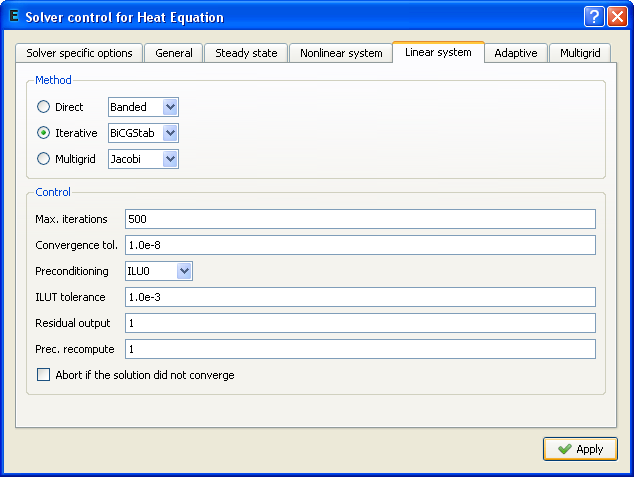
\includegraphics[scale=0.5]{images/solversettings.png}
\caption{Solver settings menu.}
\end{center}
\end{figure}

It is also possible to attach an equation to a body by holding down the SHIFT-key
while double clicking one of its surfaces. A pop up menu will then appear,
listing all possible attributes that can be attached to the selection. Choose the
attributes and press Ok.

\begin{figure}[ht]
\begin{center}
 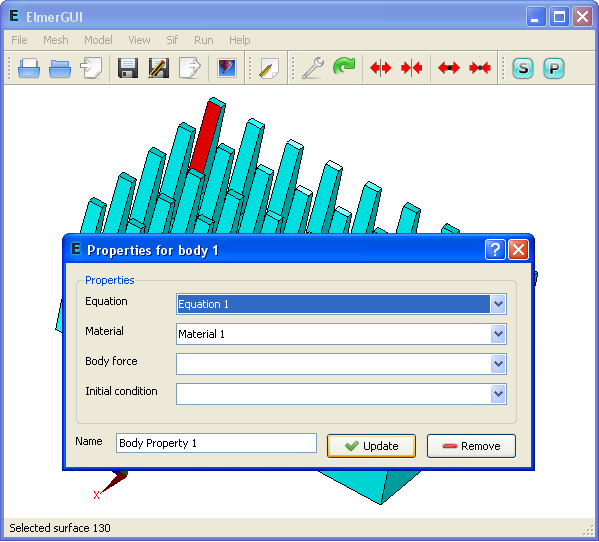
\includegraphics[scale=0.5]{images/bodyproperties.png}
\caption{Body property editor is activated by holding down the SHIFT key while double
clicking a surface.}
\end{center}
\end{figure}

\subsection{Material menu}

The next menu is related to material and model parameters:
\menu{Model}{Material}
\noindent This menu will be used to generate the ``Material'' blocks in a solver
input file.

In order to define a material parameter set and attach it to bodies, choose
\dynmenu{Model}{Material}{Add...}
\noindent 

\begin{figure}[ht]
\begin{center}
 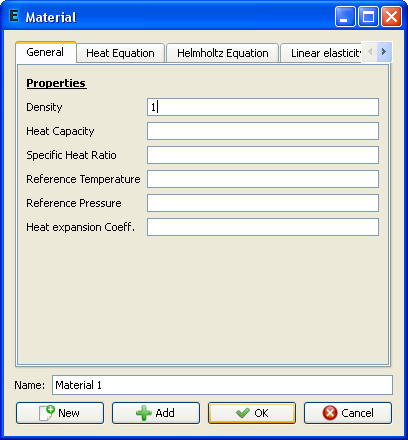
\includegraphics[scale=0.5]{images/material.png}
\caption{Material menu.}
\end{center}
\end{figure}

Again, it is possible to attach the material to a body by holding down the SHIFT-key while double clicking one of its boundaries.

\vskip2mm

{\bf Note}: The value of density should always be defined in the ``General'' tab. This
field should never be left undefined.

\vskip2mm

If you set focus in a line edit box of a dynamical menu and press Enter, a small
text edit dialog will pop up. This allows the input of more complicated expressions
than just constants. As an example, go to {\it Model $\rightarrow$ Material} and choose
{\it Add...} Place the cursor in the ``Heat conductivity'' line edit box of ``Heat
equation'' and press Enter. You can then define the heat conductivity
as a function of temperature as a piecewise linear function. An example is show in
Figure N. In this case, the heat conductivity gets value 10 if the temperature is less
than 273 degrees. It then rises from 10 to 20 between 273 and 373 degrees, and
remains constant 20 above 373 degrees.

\begin{figure}[ht]
\begin{center}
 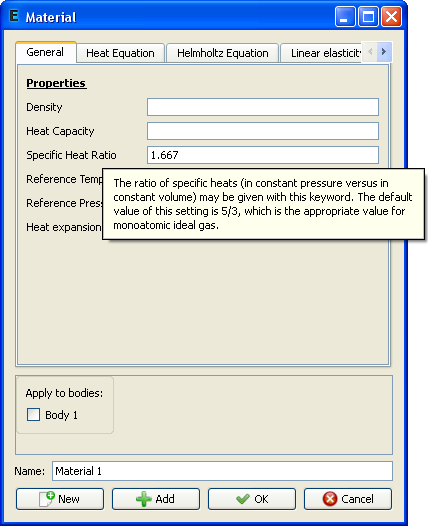
\includegraphics[scale=0.5]{images/tooltip.png}
\caption{Tooltips are shown by holding down the SHIFT and F1 keys.}
\end{center}
\end{figure}

If the user presses SHIFT and F1, a tooltip for the active widget will be displayed.

\begin{figure}[ht]
\begin{center}
 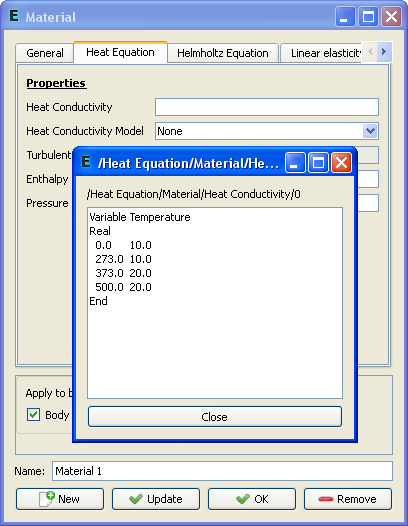
\includegraphics[scale=0.5]{images/textedit.png}
\caption{Text edit extension of a line edit box is activated by pressing Enter.}
\end{center}
\end{figure}

\subsection{Body force menu}

The next menu in the list is
\menu{Model}{Body force}
\noindent This menu is used to construct the ``Body force'' blocks in a
solver input file.

Again, choose
\dynmenu{Model}{Body force}{Add...}
\noindent to define a set of body forces and attach it to the bodies.

\begin{figure}[ht]
\begin{center}
 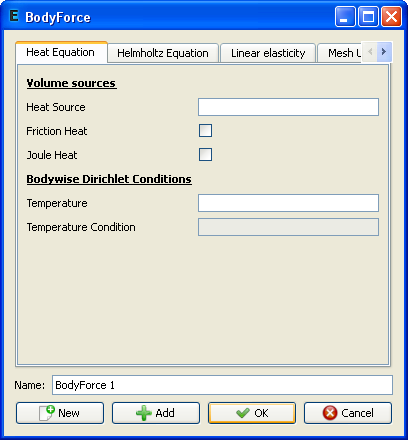
\includegraphics[scale=0.5]{images/bodyforce.png}
\caption{Body force menu.}
\end{center}
\end{figure}

\subsection{Initial condition menu}

The last menu related to body properties is
\menu{Model}{Initial condition}
\noindent 
Once again, choose
\dynmenu{Model}{Initial condition}{Add...}
\noindent to define a set of initial conditions and attach it to the bodies.

This menu is used to construct the ``Initial condition'' blocks in a
solver input file.

\begin{figure}[ht]
\begin{center}
 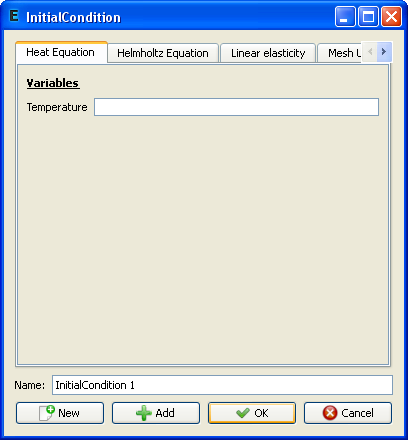
\includegraphics[scale=0.5]{images/initialcondition.png}
\caption{Initial condition menu.}
\end{center}
\end{figure}

\subsection{Boundary condition menu}

Finally, there is a menu entry for setting up the boundary conditions:
\menu{Model}{Boundary condition}
\noindent Choose
\dynmenu{Model}{Boundary condition}{Add...}
\noindent to define a set of boundary conditions and attach them to boundaries.

\begin{figure}[ht]
\begin{center}
 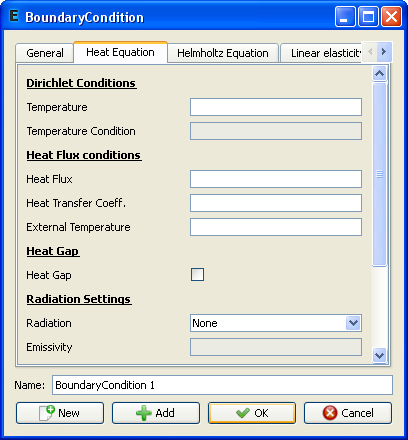
\includegraphics[scale=0.5]{images/boundarycondition.png}
\caption{Boundary condition menu.}
\end{center}
\end{figure}

It is possible to attach a boundary condition to a boundary by holding down 
the ALT or ALTGR-key while double clicking a surface or edge. A pop up menu will appear, listing all possible conditions that can be attached to the selection. 
Choose a condition from the combo box and finally press Ok.

\begin{figure}[ht]
\begin{center}
 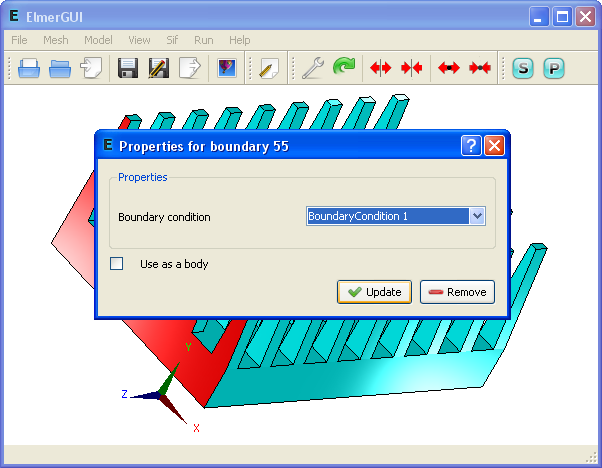
\includegraphics[scale=0.5]{images/boundaryproperties.png}
\caption{Boundary property editor activated by holding down the ALTGR key while double
clicking a surface.}
\end{center}
\end{figure}

\section{Utility functions}

\subsection{Boundary division and unification}

Some of the input file formats listed in Table 1 are not perhaps best suited for
FE-calculations, eventhough widely used. The .stl format (stereo litography format),
for example, is by definition unable to distinguish between different boundary parts
with different attributes. Moreover, the format approximates the boundary by disconnected
triangles that do not fulfill normal FE-compatibility conditions.

ElmerGUI provides a minimal set of tools for boundary division and unification. The
division is based on ``sharp edge detection''. An edge between two boundary elements
is considered sharp, if the angle between the normals exceeds a certain value (20
degrees by default). The sharp edges are then used as a mortar to divide the surface
into parts. The user may perform a sharp edge detection and boundary division from
the Mesh menu by choosing
\menu{Mesh}{Divide surface...}
\noindent In 2D the corresponding operation is
\menu{Mesh}{Divide edge...}
\noindent The resulting parts are enumerated starting from the first free index.

Sometimes, the above process produces far too many distinct parts, which eventually
need to be (re)unified. This can be done by selecting a group of surfaces by holding
down the CTRL-key while double clicking the surfaces and choosing
\menu{Mesh}{Unify surface...}
\noindent The same operation in 2D is
\menu{Mesh}{Unify edge...}
\noindent The result will inherit the smallest index from the selected group.

The sharp edges that do not belong to a closed loop may be removed by
\menu{Mesh}{Clean up}
\noindent This operation has no effect on the boundary division, but sometimes it makes
the result look better.

\subsection{Saving pictures}

The model drawn on the display area may be scanned into a 24-bit RGB image and saved in
several picture file formats:
\menu{File}{Save picture as...}
\noindent The function supports .bmp, .jpg, .png, .pbm, .pgm, and .ppm file extensions.

\subsection{View menu}

The View menu provides several utility functions for controlling the visual behaviour
of ElmerGUI. The function names should be more or less self explanatory.

\section{Solver input files}

The contents of the Model menu are passed to the solver in the form of a solver
input file. A solver input file is generated by choosing
\menu{Sif}{Generate}
\noindent The contents of the file are editable:
\menu{Sif}{Edit...}

The new sif file needs to saved before it becomes active. The recommended
method is
\menu{File}{Save project...}
\noindent In this way, also the current mesh and project files get saved in the
same directory, avoiding possible inconsistencies later on.

\section{Solution and post processing}

\subsection{Running the solver}

Once the solver input file has been generated and the project has been saved,
it is possible to actualy solve the problem:
\menu{Run}{Start solver}
\noindent This will launch either a single process for ElmerSolver (scalar solution)
or multiple MPI-processes for ElmerSolver\_mpi (parallel solution) depending on the
definitions in
\menu{Run}{Parallel settings...}

\begin{figure}[ht]
\begin{center}
 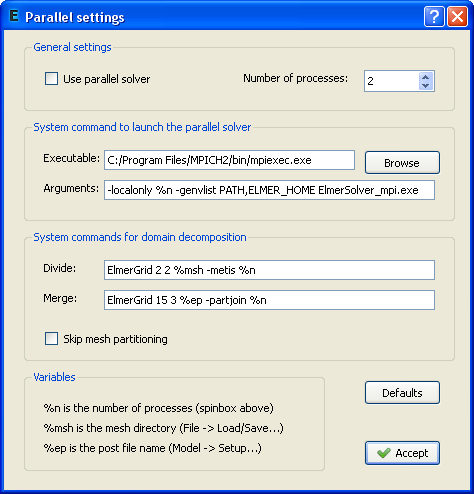
\includegraphics[scale=0.5]{images/parallelsettings.png}
\caption{Parallel settings dialog.}
\end{center}
\end{figure}

The parallel menu has three group boxes. Usually, the user is supposed to touch
only the ``General settings'' group and select the number of processes to execute.
The two remaining groups deal with system commands to launch MPI-processes and
external tools for domain decomposition.  The parallel menu is greyed out if
ElmerSolver\_mpi is not present at start-up.

When the solver is running, there is a log window and a convergence monitor
from which the iteration may be followed. In case of divergence or other troubles,
the solver may be terminated by choosing
\menu{Run}{Kill solver}

The solver will finally write a result file for ElmerPost in the project directory.
The name of the ep-file is defined in
\menu{Model}{Setup...}

\subsection{Post preocessing I (ElmerPost)}

ElmerGUI provides two different post processors for drawing, displaying, and manipulating the results.

The first alternative is activated from
\menu{Run}{Start postprocessor}
\noindent This will launch ElmerPost, which will read in the result file and displays a contour plot representing the solution. If the results were prodoced by the parallel solver, the domain decomposition used in the calculations will be shown.

\subsection{Post preocessing II (VTK)}

The second post processor is based on the Visualization Toolkit, VTK. It is activated from
\menu{Run}{Postprocessor (VTK)...}
\noindent A new window will then pop up, providing methods for drawing surfaces, contours,
vectors, and stream lines.

\subsubsection{Python interface}

If ElmerGUI has been compiled with PyhthonQt-support, there is a Python console
available for scripting. The console is located under the Edit-menu:
\menu{Edit}{PythonQt console...}
\noindent The console provides access to the following classes:
\begin{footnotesize}
\begin{verbatim}
egp             // ElmerGUI post processor
matc            // MATC language interpreter
preferences     // controls for preferences
surfaces        // controls for surface plots
vectors	        // controls for vector fields
isoContours     // controls for isocontours
isoSurfaces     // controls for isosurfaces
streamLines     // controls for streamlines
colorBar        // cotrols for the colorbar
timeStep        // controls for transient results
text            // text annotation
\end{verbatim}
\end{footnotesize}

Each of the above classes provides a number of useful methods for data and display
manipulation. To fix ideas, suppose that we want to read in the result file ``case.ep''
and display the temperature fields as a semi transparent surface plot. The commands
to execute are then the following (more examples can be found in section 7.3.3):
\begin{footnotesize}
\begin{verbatim}
py> egp.ReadPostFile("case.ep")
py> egp.SetSurfaces(True)
py> surfaces.SetFieldName("Temperature")
py> surfaces.SetOpacity(50)
py> egp.Redraw()
\end{verbatim}
\end{footnotesize}

\subsubsection{Public methods}
Interface version 0.2:
\begin{footnotesize}
\begin{verbatim}
class egp:
  bool MatcCmd(QString);                         // evaluate MATC cmd
  void domatcSlot();                             // flush MATC console

  void SetPostFileStart(int);                    // first time step
  void SetPostFileEnd(int);                      // last time step
  bool ReadPostFile(QString);                    // read result file

  void Render();                                 // render
  void ResetCamera();                            // reset camera
  void Redraw();                                 // redraw actors
  void ResetAll();                               // reset view

  void SetSurfaces(bool);                        // show/hide surfaces
  void SetVectors(bool);                         // show/hide vectors
  void SetIsoContours(bool);                     // show/hide isocontours
  void SetIsoSurfaces(bool);                     // show/hide isosurfaces
  void SetStreamLines(bool);                     // show/hide streamlines
  void SetColorBar(bool);                        // show/hide colorbar
  void SetMeshPoints(bool);                      // show/hide/nodes
  void SetMeshEdges(bool);                       // show/hide edges
  void SetFeatureEdges(bool);                    // show/hide f-edges
  void SetAxes(bool);                            // show/hide axes
  void SetText(bool);                            // show/hide text

  bool GetClipAll();                             // is clipping on?
  void SetClipAll(bool);                         // clipping on/off
  void SetClipPlaneOx(double);                   // clip plane origin
  void SetClipPlaneOy(double);                   // clip plane origin
  void SetClipPlaneOz(double);                   // clip plane origin
  void SetClipPlaneNx(double);                   // clip plane normal
  void SetClipPlaneNy(double);                   // clip plane normal
  void SetClipPlaneNz(double);                   // clip plane normal

  double GetCameraDistance();                    // get camera distance
  void SetCameraDistance(double);                // set camera distance
  double GetCameraPositionX();                   // get camera position
  double GetCameraPositionY();                   // get camera position
  double GetCameraPositionZ();                   // get camera position
  void SetCameraPositionX(double);               // set camera position
  void SetCameraPositionY(double);               // set camera position
  void SetCameraPositionZ(double);               // set camera position
  double GetCameraFocalPointX();                 // get focal point
  double GetCameraFocalPointY();                 // get focal point
  double GetCameraFocalPointZ();                 // get focal point
  void SetCameraFocalPointX(double);             // set focal point
  void SetCameraFocalPointY(double);             // set focal point
  void SetCameraFocalPointZ(double);             // set focal point
  void CameraDolly(double);                      // dolly
  void CameraRoll(double);                       // roll
  void CameraAzimuth(double);                    // azimuth
  void CameraYaw(double);                        // yaw
  void CameraElevation(double);                  // elevation
  void CameraPitch(double);                      // pitch
  void CameraZoom(double);                       // zoom
  void SetCameraRoll(double);                    // set roll
  void SetInitialCameraPosition();               // set initial position

  void RotateX(double);                          // rotate visible actors
  void RotateY(double);                          // rotate visible actors
  void RotateZ(double);                          // rotate visible actors
  void SetOrientation(double, double, double);   // set orientation
  void SetPositionX(double);                     // set position
  void SetPositionY(double);                     // set position
  void SetPositionZ(double);                     // set position
  void SetPosition(double, double, double);      // set position
  void AddPosition(double, double, double);      // add position
  void SetOrigin(double, double, double);        // set origin
  void SetScaleX(double);                        // set scale
  void SetScaleY(double);                        // set scale
  void SetScaleZ(double);                        // set scale
  void SetScale(double, double, double);         // set scale
  double GetLength();                            // get model size
  double GetNofNodes();                          // get nof nodes
  double GetMinX();                              // bounding box
  double GetMaxX();                              // bounding box
  double GetMinY();                              // bounding box
  double GetMaxY();                              // bounding box
  double GetMinZ();                              // bounding box
  double GetMaxZ();                              // bounding box

  bool SavePngFile(QString);                     // save image file

class matc:
  bool SetCommand(QString);                      // Enter MATC cmd

class preferences:
  void UseSurfaceMeshForPoints(bool);            // nodes of surface mesh
  void UseVolumeMeshForPoints(bool);             // nodes of volume mesh
  void SetPointSize(int);                        // set node point size
  void SetPointQuality(int);                     // set node point quality
  void UseClipPlaneForPoints(bool);              // clip nodes
  void UseSurfaceMeshForEdges(bool);             // edges of surface mesh
  void UseVolumeMeshForEdges(bool);              // edges of volume mesh
  void UseTubeFilterForEdges(bool);              // use tube filter
  void UseClipPlaneForEdges(bool);               // clip edges
  void SetLineWidthForEdges(int);                // edge line width
  void SetTubeQualityForEdges(int);              // edge tube quality
  void SetTubeRadiusForEdges(int);               // edge tube radius
  void UseSurfaceMeshForFeatureEdges(bool);      // surface mesh: f-edges
  void UseVolumeMeshForFeatureEdges(bool);       // volume mesh: f-edges
  void UseTubeFilterForFeatureEdges(bool);       // use tube filter
  void UseClipPlaneForFeatureEdges(bool);        // clip f-edges
  void DrawBoundaryEdges(bool);                  // draw boundary edges
  int GetFeatureAngle();                         // get feature angle
  void SetFeatureAngle(int);                     // set feature angle
  void SetLineWidthForFeatureEdges(int);         // f-edge line width
  void SetTubeQualityForFeatureEdges(int);       // f-edge tube quality
  void SetTubeRadiusForFeatureEdges(int);        // f-edge tube radius
  void SetClipPlaneOx(double);                   // clip plane origin
  void SetClipPlaneOy(double);                   // clip plane origin
  void SetClipPlaneOz(double);                   // clip plane origin
  void SetClipPlaneNx(double);                   // clip plane normal
  void SetClipPlaneNy(double);                   // clip plane normal
  void SetClipPlaneNz(double);                   // clip plane normal

class surfaces:
  QString GetFieldName();                        // get field name
  bool SetFieldName(QString);                    // set field name
  void SetMinVal(double);                        // set minimum
  void SetMaxVal(double);                        // set maximum
  void KeepLimits(bool);                         // keep limits
  void SetComputeNormals(bool);                  // shade model
  void SetFeatureAngle(int);                     // feature angle
  void SetOpacity(int);                          // set opacity
  void SetClipPlane(bool);                       // set clipping

class vectors:
  QString GetFieldName();                        // get field name
  bool SetFieldName(QString);                    // set field name
  void SetMinVal(double);                        // set minimum
  void SetMaxVal(double);                        // set maximum
  void KeepLimits(bool);                         // keep limits
  void SetComputeNormals(bool);                  // shade model
  void SetFeatureAngle(int);                     // feature angle
  void SetOpacity(int);                          // set opacity
  void SetClipPlane(bool);                       // set clipping

class isoContours:
  QString GetFieldName();                        // get field name
  QString GetColorName();                        // get color name
  bool SetFieldName(QString);                    // set field name
  bool SetColorName(QString);                    // set color name
  void SetMinFieldVal(double);                   // set min value
  void SetMaxFieldVal(double);                   // set max value
  void SetContours(int);                         // set nof contours
  void KeepFieldLimits(bool);                    // keep limits
  void SetMinColorVal(double);                   // set color min
  void SetMaxColorVal(double);                   // set color max
  void KeepColorLimits(bool);                    // keep color limits
  void UseTubeFilter(bool);                      // use tube filter
  void UseClipPlane(bool);                       // set clipping on/off
  void SetLineWidth(int);                        // set line width
  void SetTubeQuality(int);                      // set tube quality
  void SetTubeRadius(int);                       // set tube radius

class isoSurfaces:
  QString GetFieldName();                        // get field name
  QString GetColorName();                        // get color name
  bool SetFieldName(QString);                    // set field name
  bool SetColorName(QString);                    // set color name
  void SetMinFieldVal(double);                   // set min value
  void SetMaxFieldVal(double);                   // set max value
  void SetContours(int);                         // nof contours
  void KeepFieldLimits(bool);                    // keep limits
  void SetMinColorVal(double);                   // set color min
  void SetMaxColorVal(double);                   // set color max
  void KeepColorLimits(bool);                    // keep color limits
  void ComputeNormals(bool);                     // shade model
  void UseClipPlane(bool);                       // set clpping on/off
  void SetFeatureAngle(int);                     // set feature angle
  void SetOpacity(int);                          // set opacity

class streamLines:
  QString GetFieldName();                        // get field name
  QString GetColorName();                        // get color name
  bool SetFieldName(QString);                    // set field name
  bool SetColorName(QString);                    // set color name
  void SetMaxTime(double);                       // max time
  void SetStepLength(double);                    // step length
  void SetThreads(int);                          // nof threads
  void SetIntegStepLength(double);               // integ. step length
  void UseSurfaceMesh(bool);                     // use forface mesh
  void UseVolumeMesh(bool);                      // use volume mesh
  void IntegrateForwards(bool);                  // integrate forwards
  void IntegrateBackwards(bool);                 // integrate backwards
  void SetMinColorVal(double);                   // color min val
  void SetMaxColorVal(double);                   // color max value
  void KeepColorLimits(bool);                    // keep color limits
  void DrawLines(bool);                          // draw using lines
  void DrawRibbons(bool);                        // draw using ribbons
  void SetLineWidth(int);                        // line width
  void SetRibbonWidth(int);                      // ribbon width
  void UseSphereSource(bool);                    // use sphere source
  void UseLineSource(bool);                      // use line source
  void UsePointSource(bool);                     // use point source
  void SetSphereSourceX(double);                 // sphere origin
  void SetSphereSourceY(double);                 // sphere origin
  void SetSphereSourceZ(double);                 // sphere origin
  void SetSphereSourceRadius(double);            // sphere radius
  void SetSphereSourcePoints(int);               // nof pts in sphere
  void SetLineSourceStartX(double);              // line start point
  void SetLineSourceStartY(double);              // line start point
  void SetLineSourceStartZ(double);              // line start point
  void SetLineSourceEndX(double);                // line end point
  void SetLineSourceEndY(double);                // line end point
  void SetLineSourceEndZ(double);                // line end point
  void SetLineSourcePoints(int);                 // nof pts on line

class colorBar:
  bool SetFieldName(QString);                    // set field name
  void UseHorizontalLayout(bool);                // horizontal layout
  void UseVerticalLayout(bool);                  // vertical layout
  void AnnotateFieldName(bool);                  // annotate field name
  void SetLabels(int);                           // set nof labels
  void SetLineWidth(double);                     // set line width
  void SetLength(double);                        // set bar length

class timeStep:
  void SetCurrent(int);                          // set current step
  void SetStart(int);                            // set first step
  void SetStop(int);                             // set last step
  void SetIncrement(int);                        // set increment
  void SetMatcCmd(QString);                      // set MATC cmd
  void RegenerateBeforeDrawing(bool);            // regenerate actors
  void SaveFrames(bool);                         // save frames
  void SetSaveDirectory(QString);                // set save dir
  void Loop();                                   // toggle looping
  bool IsLooping();                              // is loop on?
  void DrawCurrent();                            // draw current frame

class text:
  void SetMessage(QString);                      // set annotation
  void SetPosX(int);                             // set x-position
  void SetPosy(int);                             // set y-position
\end{verbatim}
\end{footnotesize}

\subsubsection{Example scripts}

The exampels below are executed from the PythonQt-console as
\begin{footnotesize}
\begin{verbatim}
py> execfile("sample.py")
\end{verbatim}
\end{footnotesize}
where ``sample.py'' is a text file containing the script to run.

\vskip5mm
\noindent{\bf Read in results}
\begin{footnotesize}
\begin{verbatim}
egp.ReadPostFile("case.ep")
\end{verbatim}
\end{footnotesize}

\vskip5mm
\noindent{\bf Set orientation}
\begin{footnotesize}
\begin{verbatim}
egp.ReadPostFile("case.ep")
egp.SetSurfaces(True)
egp.SetOrientation(45, 45, 0)
egp.SetInitalCameraPosition()
\end{verbatim}
\end{footnotesize}

\vskip5mm
\noindent{\bf Visualize temperature on surfaces}
\begin{footnotesize}
\begin{verbatim}
egp.ReadPostFile("case.ep")
egp.SetSurfaces(True)
egp.SetOrientation(45, 45, 0)
egp.SetInitalCameraPosition()
surfaces.SetFieldName("Temperature")
egp.Redraw()
\end{verbatim}
\end{footnotesize}


\vskip5mm
\noindent{\bf Rotate object}
\begin{footnotesize}
\begin{verbatim}
import time
egp.ReadPostFile("case.ep")
egp.SetSurfaces(True)
for i in range (180):
        egp.RotateY(2.0)
        egp.ResetCamera()
        egp.Render()
        time.sleep(0.1)
\end{verbatim}
\end{footnotesize}


\vskip5mm
\noindent{\bf Traveling isosurface}
\vskip5mm
\noindent The following script makes an iso surface ($z=const.$) travel through the model
in 100 steps. The surface is colored according to the temperature field. The model it self
is drawn transparent.
\begin{footnotesize}
\begin{verbatim}
import time
egp.ReadPostFile("case.ep")
egp.SetSurfaces(True)
egp.SetIsoSurfaces(True)
egp.SetFeatureEdges(True)
preferences.SetFeatureAngle(45)
surfaces.SetFieldName("Null")
surfaces.SetOpacity(20)
isoSurfaces.SetFieldName("nodes_z")
isoSurfaces.SetColorName("Temperature")
isoSurfaces.SetContours(1)
isoSurfaces.KeepFieldLimits(True)
egp.SetOrientation(45, 45, 0)
egp.ResetCamera()
egp.Render()
zmin = egp.GetMinZ()
zmax = egp.GetMaxZ()
for i in range(100):
    z = zmin+(float(i)/100.0)*(zmax-zmin)
    isoSurfaces.SetMinFieldVal(z)
    isoSurfaces.SetMaxFieldVal(z)
    egp.Redraw()
    time.sleep(0.05)
\end{verbatim}
\end{footnotesize}


\vskip5mm
\noindent{\bf Rotate and save frames}
\begin{footnotesize}
\begin{verbatim}
egp.ReadPostFile("case.ep")
egp.SetSurfaces(True)
for i in range (180):
        egp.RotateY(2.0)
        egp.ResetCamera()
        egp.Render()
        egp.SavePngFile("frame" + str(i) + ".png")
\end{verbatim}
\end{footnotesize}

\vskip5mm
\noindent{\bf Preparing and playing back video clips}

\vskip5mm

\noindent With ffmpeg (see ffmpeg's manuals for more accurate controls):
\begin{footnotesize}
\begin{verbatim}
$ ffmpeg -b 1000000 -i frame%d.png example.avi
\end{verbatim}
\end{footnotesize}
With mencoder (see mencoder's manuals for better controls):
\begin{footnotesize}
\begin{verbatim}
$ mencoder -ovc lavc -mf type=png:fps=25 -o example.avi mf://frame%d.png
\end{verbatim}
\end{footnotesize}
Playback with mplayer (choose appropriate frame rate):
\begin{footnotesize}
\begin{verbatim}
$ mplayer -fps 50 example.avi
\end{verbatim}
\end{footnotesize}

\subsubsection{ECMAScript interface}

In addition to Python, it is possible to use Qt's internal ECMAScript engine for scripting. The ECMAScript console is activated from
the Edit menu as:
\menu{Edit}{ECMAScript console...}
The ECMAScript interface provides access to the same classes and methods
as the Python interface. However, users familiar with e.g. JavaScript (from
which ECMAScript has been derived and standardized) may find the ECMAScript interface more comfortable.

ECMAScript files are executed from the console by entering the command
\begin{footnotesize}
\begin{verbatim}
qs> egp.Execute("script.qs")
\end{verbatim}
\end{footnotesize}

The above examples for Python translate to the following ECMAScript files:

\vskip5mm
\noindent{\bf Read in results}
\begin{footnotesize}
\begin{verbatim}
egp.ReadPostFile("case.ep")
\end{verbatim}
\end{footnotesize}

\vskip5mm
\noindent{\bf Set orientation}
\begin{footnotesize}
\begin{verbatim}
egp.ReadPostFile("case.ep")
egp.SetSurfaces(true)
egp.SetOrientation(45, 45, 0)
egp.SetInitalCameraPosition()
\end{verbatim}
\end{footnotesize}

\vskip5mm
\noindent{\bf Visualize temperature on surfaces}
\begin{footnotesize}
\begin{verbatim}
egp.ReadPostFile("case.ep")
egp.SetSurfaces(true)
egp.SetOrientation(45, 45, 0)
egp.SetInitalCameraPosition()
surfaces.SetFieldName("Temperature")
egp.Redraw()
\end{verbatim}
\end{footnotesize}

\vskip5mm
\noindent{\bf Rotate object}
\begin{footnotesize}
\begin{verbatim}
egp.ReadPostFile("case.ep")
egp.SetSurfaces(true)
for(var i = 0; i < 180; i++)
{
   egp.RotateY(2.0)
   egp.ResetCamera()
   egp.Render()
}
\end{verbatim}
\end{footnotesize}

\vskip5mm
\noindent{\bf Traveling isosurface}
\begin{footnotesize}
\begin{verbatim}
egp.ReadPostFile("case.ep")
egp.SetSurfaces(true)
egp.SetIsoSurfaces(true)
egp.SetFeatureEdges(true)
preferences.SetFeatureAngle(45)
surfaces.SetFieldName("Null")
surfaces.SetOpacity(20)
isoSurfaces.SetFieldName("nodes_z")
isoSurfaces.SetColorName("Temperature")
isoSurfaces.SetContours(true)
isoSurfaces.KeepFieldLimits(true)
egp.SetOrientation(45, 45, 0)
egp.ResetCamera()
egp.Render()
var zmin = egp.GetMinZ()
var zmax = egp.GetMaxZ()
for(var i = 0; i < 100; i++)
{
   var z = zmin + i/100.0 * (zmax-zmin)
   isoSurfaces.SetMinFieldVal(z)
   isoSurfaces.SetMaxFieldVal(z)
   egp.Redraw()
}
\end{verbatim}
\end{footnotesize}

\vskip5mm
\noindent{\bf Rotate and save frames}
\begin{footnotesize}
\begin{verbatim}
egp.ReadPostFile("case.ep")
egp.SetSurfaces(true)
for(var i = 0; i < 180; i++)
{
    egp.RotateY(2.0)
    egp.ResetCamera()
    egp.Render()
    egp.SavePngFile("frame" + i + ".png")
}
\end{verbatim}
\end{footnotesize}


\bibliographystyle{plain}
\bibliography{elmergui}

\appendix

\section{ElmerGUI initialization file}

The initialization file for ElmerGUI is located in {\tt ELMERGUI\_HOME/edf}. It is called {\tt egini.xml}:

\begin{footnotesize}
\begin{verbatim}
<?xml version='1.0' encoding='UTF-8'?>
<!DOCTYPE egini>
<egini version="1.0">

  Show splash screen at startup:
  <splashscreen> 1 </splashscreen>

  Show system tray icon:
  <systrayicon> 1 </systrayicon>

  Show system tray messages:
  <systraymessages> 1 </systraymessages>

  System tray message duration in millisecons:
  <systraymsgduration> 3000 </systraymsgduration>

  Check the presence of external components:
  <checkexternalcomponents> 0 </checkexternalcomponents>

  Hide toolbars:
  <hidetoolbars> 0 </hidetoolbars>

  Plot convergence view:
  <showconvergence> 1 </showconvergence>

  Draw background image:
  <bgimage> 1 </bgimage>

  Background image file:
  <bgimagefile> :/images/bgimage.png </bgimagefile>

  Align background image to the bottom right corner of the screen:
  <bgimagealignright> 0 </bgimagealignright>

  Stretch background image to fit the display area (overrides align):
  <bgimagestretch> 1 </bgimagestretch>

  Maximum number of solvers / equation:
  <max_solvers> 10 </max_solvers>

  Maximum number of equations:
  <max_equations> 10 </max_equations>

  Maximum number of materials:
  <max_materials> 10 </max_materials>

  Maximum number of bodyforces:
  <max_bodyforces> 10 </max_bodyforces>

  Maximum number of initial conditions:
  <max_initialconditions> 10 </max_initialconditions>

  Maximum number of bodies:
  <max_bodies> 100 </max_bodies>

  Maximum number of bcs:
  <max_bcs> 500 </max_bcs>

  Maximum number of boundaries:
  <max_boundaries> 500 </max_boundaries>

</egini>
\end{verbatim}
\end{footnotesize}

You may change the default behaviour of ElmerGUI by editing this file. For example, to turn off the splash screen at start up, change the value of the tag {\tt <splshscreen>} from 1 to 0. To change the background image, enter a picture file name in the {\tt <bgimagefile>} tag. You might also want to increase the default values for solvers, equations, etc., in case of very complex models.

\section{ElmerGUI material database}

The file {\tt ELMERGUI\_HOME/edf/egmaterials.xml} defines the material database for ElmerGUI. The
format of this file is the following:

\begin{footnotesize}
\begin{verbatim}
 
<!DOCTYPE egmaterials>
<materiallibrary>
  
  <material name="Air (room temperature)" >
    <parameter name="Density" >1.205</parameter>
    <parameter name="Heat conductivity" >0.0257</parameter>
    <parameter name="Heat capacity" >1005.0</parameter>
    <parameter name="Heat expansion coeff." >3.43e-3</parameter>
    <parameter name="Viscosity" >1.983e-5</parameter>
    <parameter name="Turbulent Prandtl number" >0.713</parameter>
    <parameter name="Sound speed" >343.0</parameter>
  </material>

  <material name="Water (room temperature)" >
    <parameter name="Density" >998.3</parameter>
    <parameter name="Heat conductivity" >0.58</parameter>
    <parameter name="Heat capacity" >4183.0</parameter>
    <parameter name="Heat expansion coeff." >0.207e-3</parameter>
    <parameter name="Viscosity" >1.002e-3</parameter>
    <parameter name="Turbulent Prandtl number" >7.01</parameter>
    <parameter name="Sound speed" >1497.0</parameter>
  </material>
  ...
</materiallibrary>

\end{verbatim}
\end{footnotesize}

The values of the parameters may be either constant, or functions of time, temperature, etc.
A temperature dependent parameter may be defined e.g. as

\begin{footnotesize}
\begin{verbatim}
<parameter name="A" >Variable Temperature; Real; 2 3; 4 5; End</parameter>
\end{verbatim}
\end{footnotesize}
In this case, $A(2)=3$ and $A(4)=5$. Values between the points are interpolated linearly,
and extrapolated in the tangent direction outside the domain. The number of points defining 
he interpolant may be arbitrary. 

\section{ElmerGUI definition files}

The directory {\tt ELMERGUI\_HOME} contains a subdirectory called ``edf''. This is the place where all ElmerGUI definition files (ed-files) reside. The definition files are XML-formatted text files which define the contents and appearance of the Model menu.

The ed-files are loaded iteratively from the edf-directory once and for all when ElmerGUI starts. Later, it is possible to view and edit their contents by choosing
\menu{File}{Definitions...}

An ed-file has the following structure:
\begin{footnotesize}
\begin{verbatim}
<?xml version='1.0' encoding='UTF-8'?>
<!DOCTYPE edf>
<edf version="1.0">
   [PDE block]
   [PDE block]
   ...
   [PDE block]
</edf>
\end{verbatim}
\end{footnotesize}

The structure of a [PDE block] is the following:
\begin{footnotesize}
\begin{verbatim}
<PDE Name="My equation">
   <Name>
      My equation
   </Name>
   ...
   <Equation>
      [Widget block]
   </Equation>
   ...
   <Material>
      [Widget block]
   </Material>
   ...
   <BodyForce>
      [Widget block]
   <BodyForce>
   ...
   <InitialCondition>
      [Widget block]
   </InitialCondition>
   ...
   <BoundaryCondition>
      [Widget block]
   </BoundaryCondition>
</PDE>
\end{verbatim}
\end{footnotesize}
Note that the name of the PDE is defined redundantly in two occurances.

The basic stucture of a [Widget block] is the following:
\begin{footnotesize}
\begin{verbatim}
<Parameter Widget="Label">
   <Name> My label </Name>
</Parameter>
...
<Parameter Widget="Edit"> 
   <Name> My edit box </Name>
   <Type> Integer </Type>
   <Whatis> Meaning of my edit box </Whatis>
</Parameter>
...
<Parameter Widget="CheckBox">
   <Name> My check box </Name>
   <Type> Logical </Type>
   <Whatis> Meaning of my check box </Whatis>
</Parameter>
...
<Parameter Widget="Combo"> 
   <Name> My combo box </Name> 
   <Type> String </Type>
   <Item> <Name> My 1st item </Name> </Item>
   <Item> <Name> My 2nd item </Name> </Item>
   <Item> <Name> My 3rd item </Name> </Item>
   <Whatis> Meaning of my combo box </Whatis>
</Parameter>
\end{verbatim}
\end{footnotesize}

There are four types of widgets available:
\begin{itemize}
 \item Label (informative text)
 \item CheckBox (switches)
 \item ComboBox (selection from list)
 \item LineEdit (generic variables)
\end{itemize}
Each widget must be given a name and and a variable type: logical, integer, real, or  string. It is also a good practice to equip the widgets with tooltips explaining their purpose and meaning as clearly as possible.

Below is a working example of a minimal ElmerGUI definition file. It will add ``My equation'' to the equation tabs in the Model menu, see Figure N. The file is called ``sample.edf'' and it should be placed in {\tt ELMERGUI\_HOME/edf}.

\begin{footnotesize}
\begin{verbatim}
<?xml version='1.0' encoding='UTF-8'?>
<!DOCTYPE edf>
<edf version="1.0">
  <PDE Name="My equation">
    <Name> My equation </Name>
    <Equation>
      <Parameter Widget="Label">
        <Name> My label </Name>
      </Parameter>
      <Parameter Widget="Edit">
        <Name> My edit box </Name>
        <Type> Integer </Type>
        <Whatis> Meaning of my edit box </Whatis>
      </Parameter>
      <Parameter Widget="CheckBox">
        <Name> My check box </Name>
        <Type> Logical </Type>
        <Whatis> Meaning of my check box </Whatis>	  
      </Parameter>
      <Parameter Widget="Combo">
        <Name> My combo box </Name>
        <Type> String </Type>
        <Item> <Name> My 1st item </Name> </Item>
        <Item> <Name> My 2nd item </Name> </Item>
        <Item> <Name> My 3rd item </Name> </Item>
        <Whatis> Meaning of my combo box </Whatis>	  
      </Parameter>
    </Equation>
  </PDE>
</edf>
\end{verbatim}
\end{footnotesize}

\begin{figure}[ht]
\begin{center}
 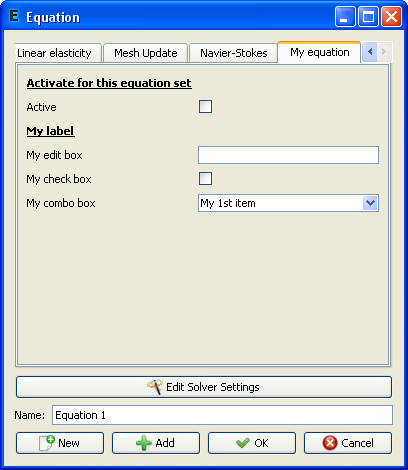
\includegraphics[scale=0.5]{images/edfsample.png}
\caption{Equation tab in Model menu produced by the sample ed-file.}
\end{center}
\end{figure}

More sophisticated examples with different tags and attribites can be found from the XML-files in  {\tt ELMERGUI\_HOME/edf}.

\newpage

\section{Elmer mesh files}

\noindent {\bf mesh.header}
\begin{verbatim}
nodes elements boundary-elements
types
type1 elements1
type2 elements2
...
typeN elementsN
\end{verbatim}

\vskip5mm

\noindent {\bf mesh.nodes}
\begin{verbatim}
node1 tag1 x1 y1 z1
node2 tag2 x2 y2 z2
...
nodeN tagN xN yN zN
\end{verbatim}

\vskip5mm

\noindent {\bf mesh.elements}
\begin{verbatim}
element1 body1 type1 n11 ... n1M
element2 body2 type2 n21 ... n2M
...
elementN bodyN typeN nN1 ... nNM
\end{verbatim}

\vskip5mm

\noindent {\bf mesh.boundary}
\begin{verbatim}
element1 boundary1 parent11 parent12 n11 ... n1M
element2 boundary2 parent21 parent22 n21 ... n2M
...
elementN boundaryN parentN1 parentN2 nN1 ... nNM
\end{verbatim}

\newpage

\section{Adding menu entries to ElmerGUI}

As ElmerGUI is based on Qt4, it should be relatively easy to customize the menus
and dialog windows. A new menu item, for example, is added as follows.

First, we declare the menu action and a private slot in {\tt src/mainwindow.h}:
\begin{verbatim}
private slots:
   ...
   void mySlot();
   ...

private:
   ...
   QAction *myAct;
   ...
\end{verbatim}

Then, in {\tt src/mainwindow.cpp}, we actually create the action, connect
an appropriate signal from the action to the slot, and add the action in
a menu:
\begin{verbatim}
void MainWindow::createActions()
{
   ...
   myAct = new QAction(tr("*** My menu entry ***"), this);
   connect(myAct, SIGNAL(triggered()), this, SLOT(mySlot()));
   ...
}
\end{verbatim}
and
\begin{verbatim}
void MainWindow::createMenus()
{
   ...
   meshMenu->addSeparator();
   meshMenu->addAction(myAct);
   ...
}
\end{verbatim}

It finally remains to define the slot to which the triggering signal is connected.
All processing related to the action should be done here:
\begin{verbatim}
void MainWindow::mySlot()
{
   cout << "Here we go!" << endl;
}
\end{verbatim}

\newpage

\section{ElmerGUI mesh structure}

The finite element mesh generated by ElmerGUI is of class {\tt mesh\_t}
(declared in {\tt src/meshtype.h}). The mesh is private to the class {\tt GLWidget}
(declared in {\tt src/glwidget.h}), which is responsible of drawing and
rendering the model.

\subsection{GLWidget}

The class {\tt GLWidget} provides the following public methods for accessing the mesh:
\begin{verbatim}
mesh_t* GLWidget::getMesh()
\end{verbatim}
Get the active mesh.
\begin{verbatim}
void GLWidget::newMesh()
\end{verbatim}
Allocate space for a new mesh.
\begin{verbatim}
void GLWidget::deleteMesh()
\end{verbatim}
Delete the current mesh.
\begin{verbatim}
bool GLWidget::hasMesh()
\end{verbatim}
Returns true if there is a mesh. Otherwise returns false.
\begin{verbatim}
void GLWidget::setMesh(mesh_t* myMesh)
\end{verbatim}
Set active mesh to myMesh.

The mesh can be accessed in {\tt MainWindow} for example as follows
(see previous section for more details):
\begin{verbatim}
void MainWindow::mySlot()
{
   if(!glWidget->hasMesh()) return;
   mesh_t* mesh = glWidget->getMesh();
   cout << "Nodes: " << mesh->getNodes() << endl;
   cout << "Edges: " << mesh->getEdges() << endl;
   cout << "Trias: " << mesh->getSurfaces() << endl;
   cout << "Tetras: " << mesh->getElements() << endl;
}
\end{verbatim}

\subsection{mesh\_t}

The class {\tt mesh\_t} provides the following public methods for accessing
and manipulating mesh data:
\begin{verbatim}
bool mesh_t::isUndefined()
\end{verbatim}
Returns true if the mesh is undefined. Otherwise returns false.
\begin{verbatim}
void mesh_t::clear()
\end{verbatim}
Clears the current mesh.
\begin{verbatim} 
bool mesh_t::load(char* dir)
\end{verbatim}
Loads Elmer mesh files from directory dir. Returns false if loading failed. Otherwise returns true.
\begin{verbatim} 
bool mesh_t::save(char* dir)
\end{verbatim}
Saves the mesh in Elmer format in directory dir. Returns false if saving failed. Otherwise returns true.
\begin{verbatim} 
double* mesh_t::boundingBox()
\end{verbatim}
Returns bounding box for the current mesh (xmin, xmax, ymin, ymax, zmin, zmax, xmid, ymid, zmid, size).
\begin{verbatim} 
void mesh_t::setCdim(int cdim)
\end{verbatim}
Set coordinate dimension to cdim.
\begin{verbatim}  
int mesh_t::getCdim()
\end{verbatim}
Get coordinate dimension for the current mesh.
\begin{verbatim}  
void mesh_t::setDim(int dim)
\end{verbatim}
Set mesh dimension to dim.
\begin{verbatim}
int mesh_t::getDim()
\end{verbatim}
Get mesh dimension.
\begin{verbatim}  
void mesh_t::setNodes(int n)
\end{verbatim}
Set the number of nodes to n.
\begin{verbatim} 
int mesh_t::getNodes()
\end{verbatim}
Get the number of nodes.
\begin{verbatim} 
void mesh_t::setPoints(int n)
\end{verbatim}
Set the number of point elements to n.
\begin{verbatim} 
int mesh_t::getPoints()
\end{verbatim}
Get the number of point elements.
\begin{verbatim} 
void mesh_t::setEdges(int n)
\end{verbatim}
Set the number of edge elements to n.
\begin{verbatim}   
int mesh_t::getEdges()
\end{verbatim}
Get the number of edge elements.
\begin{verbatim} 
void mesh_t::setSurfaces(int n)
\end{verbatim}
Set the number of surface elements to n.
\begin{verbatim} 
int mesh_t::getSurfaces()
\end{verbatim}
Get the number of surface elements.
\begin{verbatim} 
void mesh_t::setElements(int n)
\end{verbatim}
Set the number of volume elements to n.
\begin{verbatim} 
int mesh_t::getElements()
\end{verbatim}
Get the number of volume elements.
\begin{verbatim} 
node_t* mesh_t::getNode(int n)
\end{verbatim}
Get node n.
\begin{verbatim} 
void mesh_t::setNodeArray(node_t* nodeArray)
\end{verbatim}
Set node array point to nodeArray. Useful, if the user wants to take care of memory allocation by him/her self.
\begin{verbatim} 
void mesh_t::newNodeArray(int n)
\end{verbatim}
Allocate memory for n nodes.
\begin{verbatim}
void mesh:t::deleteNodeArray()
\end{verbatim}
Delete current node array.
\begin{verbatim}
point_t* mesh_t::getPoint(int n)
\end{verbatim}
Get point element n.
\begin{verbatim}
void mesh_t::setPointArray(point_t* pointArray)
\end{verbatim}
Set point element array point to pointArray. Useful, if the user wants to take care of memory allocation by him/her self.
\begin{verbatim} 
void mesh_t::newPointArray(int n)
\end{verbatim}
Allocate memory for n point elements.
\begin{verbatim}
void mesh_t::deletePointArray()
\end{verbatim}
Delete current point element array.
\begin{verbatim}
edge_t* mesh_t::getEdge(int n)
\end{verbatim}
Get edge element n.
\begin{verbatim}
void mesh_t::setEdgeArray(edge_t* edgeArray)
\end{verbatim}
Set edge element array point to edgeArray. Useful, if the user wants to take care of memory allocation by him/her self.
\begin{verbatim} 
void mesh_t::newEdgeArray(int n)
\end{verbatim}
Allocate memory for n edge elements.
\begin{verbatim}
void mesh_t::deleteEdgeArray()
\end{verbatim}
Delete current edge elemet array.
\begin{verbatim}
surface_t* mesh_t::getSurface(int n)
\end{verbatim}
Get surface element n.
\begin{verbatim}
void mesh_t::setSurfaceArray(surface_t* surfaceArray)
\end{verbatim}
Set surface element array point to surfaceArray. Useful, if the user wants to take care of memory allocation by him/her self.
\begin{verbatim} 
void mesh_t::newSurfaceArray(int n);
\end{verbatim}
Allocate memory for n surface elements.
\begin{verbatim}
void mesh_t::deleteSurfaceArray()
\end{verbatim}
Delete surface element array.
\begin{verbatim}
element_t* mesh_t::getElement(int n)
\end{verbatim}
Get volume element n.
\begin{verbatim}
void mesh_t::setElementArray(element_t* elementArray)
\end{verbatim}
Set volume element array point to elementArray. Useful, if the user wants to take care of memory allocation by him/her self.
\begin{verbatim} 
void mesh_t::newElementArray(int n)
\end{verbatim}
Allocate memory for n volume elements.
\begin{verbatim} 
void mesh_t::deleteElementArray()
\end{verbatim}
Delete current volume element array.

\subsection{node\_t}

The class {\tt node\_t} has been declared in {\tt src/meshtypes.h}. It provides the
following public methods for accessing node data:
\begin{verbatim}
void node_t::setX(int n, double x)
\end{verbatim}
Set component n of the position vector to x.
\begin{verbatim} 
double node_t::getX(int n)
\end{verbatim}
Get component n of the position vector.
\begin{verbatim} 
void node_t::setXvec(double* v)
\end{verbatim}
Set the position vector to v.
\begin{verbatim} 
double* node_t::getXvec()
\end{verbatim}
Get the position vector.
\begin{verbatim}
void node_t::setIndex(int n)
\end{verbatim}
Set the index of the node to n.
\begin{verbatim} 
int node_t::getIndex()
\end{verbatim}
Get the index of the node.

\subsection{Base element class element\_t}

The class {\tt element\_t} provides the following methods for accessing element data:
\begin{verbatim} 
void element_t::setNature(int n)
\end{verbatim}
Set element nature to n (either PDE\_UNKNOWN, PDE\_BOUNDARY, or PDE\_BULK).
\begin{verbatim}
int element_t::getNature()
\end{verbatim}
Get the element nature.
\begin{verbatim}
void element_t::setCode(int n)
\end{verbatim}
Set element code to n (202 = two noded line, 303 = three noded triangle, ...)
\begin{verbatim}
int element_t::getCode()
\end{verbatim}
Get the element code.
\begin{verbatim}
void element_t::setNodes(int n)
\end{verbatim}
Set the number of nodes to n.
\begin{verbatim}
int element_t::getNodes()
\end{verbatim}
Get the number of nodes.
\begin{verbatim}
void element_t::setIndex(int n)
\end{verbatim}
Set element index to n.
\begin{verbatim}
int element_t::getIndex()
\end{verbatim}
Get the element index.
\begin{verbatim}
void element_t::setSelected(int n)
\end{verbatim}
Set the selection state (1=selected, 0=unselected).
\begin{verbatim}
int element_t::getSelected()
\end{verbatim}
Returns 1 if element is selected. Otherwise returns 0.
\begin{verbatim}
int element_t::getNodeIndex(int n)
\end{verbatim}
Get the index of node n.
\begin{verbatim}
void element_t::setNodeIndex(int m, int n)
\end{verbatim}
Set the index of node m to n.
\begin{verbatim}
int* element_t::getNodeIndexes()
\end{verbatim}
Get the indexes of all nodes.
\begin{verbatim}
void element_t::newNodeIndexes(int n)
\end{verbatim}
Allocate space for n node indexes.
\begin{verbatim}
void element_t::deleteNodeIndexes()
\end{verbatim}
Delete all node indexes.

\subsection{Point element class point\_t}

The class {\tt point\_t} inherits all public members from class {\tt element\_t}.
In addition to this, it provides the following methods for accessing and
manipulating point element data:
\begin{verbatim}
void setSharp(bool b);
\end{verbatim}
Mark the point element ``sharp'' (b=true) or not (b=false).
\begin{verbatim}
bool isSharp();
\end{verbatim}
Returns true if the point element is ``sharp''. Otherwise returns false.
\begin{verbatim}
void setEdges(int n);
\end{verbatim}
Set the number of edges elements connected to the point to n.
\begin{verbatim}
int getEdges();
\end{verbatim}
Get the number of edge elements connected to the point.
\begin{verbatim}
void setEdgeIndex(int m, int n);
\end{verbatim}
Set the index of m'th edge element to n.
\begin{verbatim}
int getEdgeIndex(int n);
\end{verbatim}
Get the index of n'th connected edge element.
\begin{verbatim}
void newEdgeIndexes(int n);
\end{verbatim}
Allocate space for n edge element indexes.
\begin{verbatim}
void deleteEdgeIndexes();
\end{verbatim}
Delete all edge element indexes.

\subsection{Edge element class edge\_t}

The class {\tt edge\_t} inherits all public methods from {\tt element\_t}.
It also provides the following methods for accessing and manipulating edge
element data:
\begin{verbatim}
void edge_t::setSharp(bool b)
\end{verbatim}
Mark the edge sharp (b=true) or not (b=false).
\begin{verbatim}
bool edge_t::isSharp()
\end{verbatim}
Returns true if the edge is sharp.
\begin{verbatim} 
void edge_t::setPoints(int n)
\end{verbatim}
Set the number of point elements connected to the edge to n.
\begin{verbatim}
int edge_t::getPoints()
\end{verbatim}
Get the number of point elements connected to the edge.
\begin{verbatim}
void edge_t::setPointIndex(int m, int n)
\end{verbatim}
Set the index of point element m to n.
\begin{verbatim}
int edge_t::getPointIndex(int n)
\end{verbatim}
Get the index of point element n.
\begin{verbatim}
void edge_t::newPointIndexes(int n)
\end{verbatim}
Allocate space for n point element indexes.
\begin{verbatim}
void edge_t::deletePointIndexes()
\end{verbatim}
Delete all point element indexes.
\begin{verbatim}
void edge_t::setSurfaces(int n)
\end{verbatim}
Set the number of surface elements connected to the edge to n.
\begin{verbatim}
int edge_t::getSurfaces()
\end{verbatim}
Get the number of surface elements connected to the edge.
\begin{verbatim}
void edge_t::setSurfaceIndex(int m, int n)
\end{verbatim}
Set the index of surface element m to n.
\begin{verbatim}
int edge_t::getSurfaceIndex(int n)
\end{verbatim}
Get the index of m'th surface element connected to the edge.
\begin{verbatim}
void edge_t::newSurfaceIndexes(int n)
\end{verbatim}
Allocate space for n surface element indexes.
\begin{verbatim}
void edge_t::deleteSurfaceIndexes()
\end{verbatim}
Delete all surface element indexes.

\subsection{Surface element class surface\_t}

Finally, the class {\tt surface\_t} provides the following public methods for
accessing and manipulating surface element data, besides of those inherited
from the base element class {\tt element\_t}:

\begin{verbatim}
void surface\_t::setEdges(int n)
\end{verbatim}
Set the number of edge elements connected to the surface to n.
\begin{verbatim}
int surface\_t::getEdges()
\end{verbatim}
Get the number of edge elements connected to the surface element.
\begin{verbatim}
void surface\_t::setEdgeIndex(int m, int n)
\end{verbatim}
Set the inde of m'th edge element to n.
\begin{verbatim}
int surface\_t::getEdgeIndex(int n)
\end{verbatim}
Get the index of n'th edge element connected to the surface element.
\begin{verbatim}
void surface\_t::newEdgeIndexes(int n)
\end{verbatim}
Allocate space for n edge element indexes.
\begin{verbatim}
void surface\_t::deleteEdgeIndexes()
\end{verbatim}
Delete all edge element indexes.
\begin{verbatim}
void surface\_t::setElements(int n)
\end{verbatim}
Set the number of volume elements connected to the surface element to n.
\begin{verbatim}
int surface\_t::getElements()
\end{verbatim}
Get the number of volume elements connected to the surface element.
\begin{verbatim}
void surface\_t::setElementIndex(int m, int n)
\end{verbatim}
Set the index of m'th volume element to n.
\begin{verbatim}
int surface\_t::getElementIndex(int n)
\end{verbatim}
Get the index of n'th volume element connected to the surface.
\begin{verbatim}
void surface\_t::newElementIndexes(int n)
\end{verbatim}
Allocate space for n volume element indexes.
\begin{verbatim}
void surface\_t::deleteElementIndexes()
\end{verbatim}
Delete all volume element indexes.
\begin{verbatim}
void surface\_t::setNormalVec(double* v)
\end{verbatim}
Set the normal vector to the surface element.
\begin{verbatim}
double* surface\_t::getNormalVec()
\end{verbatim}
Get the normal vector for the surface element.
\begin{verbatim}
double surface\_t::getNormal(int n)
\end{verbatim}
Get component n of the normal vector.
\begin{verbatim}
void surface\_t::setNormal(int n, double x)
\end{verbatim}
Set component n of the normal to x.
\begin{verbatim}
void surface\_t::setVertexNormalVec(int n, double* v)
\end{verbatim}
Set the normal vector for vertex n to v.
\begin{verbatim}
void surface\_t::addVertexNormalVec(int m, double* v)
\end{verbatim}
Add vector v to the normal in vertex n.
\begin{verbatim}
void surface\_t::subVertexNormalVec(int m, double* v)
\end{verbatim}
Subtract vector v from the normal in vertex n.
\begin{verbatim}
double* surface\_t::getVertexNormalVec(int n)
\end{verbatim}
Get the normal vector in vertex n.

\end{document}

